% CVPR 2025 Paper Template; see https://github.com/cvpr-org/author-kit

\documentclass[10pt,twocolumn,letterpaper]{article}

%%%%%%%%% PAPER TYPE  - PLEASE UPDATE FOR FINAL VERSION
\usepackage{cvpr}              % To produce the CAMERA-READY version
% \usepackage[review]{cvpr}      % To produce the REVIEW version
% \usepackage[pagenumbers]{cvpr} % To force page numbers, e.g. for an arXiv version
\usepackage{graphicx}
% Import additional packages in the preamble file, before hyperref
%
% --- inline annotations
%
\newcommand{\red}[1]{{\color{red}#1}}
\newcommand{\todo}[1]{{\color{red}#1}}
\newcommand{\TODO}[1]{\textbf{\color{red}[TODO: #1]}}
% --- disable by uncommenting  
% \renewcommand{\TODO}[1]{}
% \renewcommand{\todo}[1]{#1}



% It is strongly recommended to use hyperref, especially for the review version.
% hyperref with option pagebackref eases the reviewers' job.
% Please disable hyperref *only* if you encounter grave issues, 
% e.g. with the file validation for the camera-ready version.
%
% If you comment hyperref and then uncomment it, you should delete *.aux before re-running LaTeX.
% (Or just hit 'q' on the first LaTeX run, let it finish, and you should be clear).
\definecolor{cvprblue}{rgb}{0.21,0.49,0.74}
\usepackage[pagebackref,breaklinks,colorlinks,allcolors=cvprblue]{hyperref}

%%%%%%%%% PAPER ID  - PLEASE UPDATE
\def\paperID{*****} % *** Enter the Paper ID here
\def\confName{CVPR}
\def\confYear{2025}

%%%%%%%%% TITLE - PLEASE UPDATE
\title{Art Style Classification: Enhancing Accuracy with Shallow \\Neural Network Adapter}

%%%%%%%%% AUTHORS - PLEASE UPDATE
\author{Lu Yingxi\thanks{Equal contribution}\\
2023011435\\
Class 31\\
{\tt\small lu-yx23@mails.tsinghua.edu.cn}
\and
Zhu Fangyu\thanks{Equal contribution}\\
2023011410\\
Class 32\\
{\tt\small xx@mails.tsinghua.edu.cn}\\
}
\begin{document}
\twocolumn[{%
\renewcommand\twocolumn[1][]{#1}%
\maketitle

}]
\begin{abstract}
This is the abstract.
\end{abstract}    
\section{Introduction}

In this project, we aim to address the challenge of classifying paintings according to their artistic styles. This task lies at the intersection of computer vision, machine learning, and art history, making it a multifaceted problem with significant implications for both technological and cultural domains\cite{CETINIC2018107}. In recent years, the automated classification of art painting styles using deep convolutional neural networks (CNNs) has become essential for analyzing and categorizing vast digitized art collections. These models can learn hierarchical visual features directly from raw image data, providing a powerful tool for art analysis\cite{li2025enhanced}\cite{imran2023artistic}. However, accurately recognizing and distinguishing stylistic characteristics across diverse art movements remains a challenge due to high intra-class variability and inter-class similarity\cite{alkofer2021using}. Developing robust classification methods is critical for scalable digital archiving, enhancing curatorial workflows, and enabling large-scale quantitative analysis of artistic trends to support art historical research.

Our project builds upon the approach proposed in\cite{imran2023artistic}, which involves a two-stage architecture combining a deep neural network (DNN) and a shallow neural network (SNN) adapter. The DNN acts as a feature extractor, while the SNN adapter is responsible for decision-making. Each input image is divided into five distinct patches: top-left, top-right, bottom-left, bottom-right, and center. The DNN independently classifies each of these five patches, and the SNN adapter aggregates the results to produce a final classification. This architecture allows for a more detailed examination of different regions within an artwork, capturing fine-grained information and preserving important artistic details\cite{imran2023artistic}. Importantly, the SNN operates independently of the DNN, meaning that the introduction of the SNN does not alter the architecture or weights of the DNN. This independence allows the SNN to function as a flexible adapter, enhancing the classification process without imposing any architectural constraints on the DNN. Thus, the integrity and performance of the original DNN are maintained while adding an additional layer of refinement to the classification results.

By comparing the prediction results of the DNN direct output and the SNN adapter output, we observed that while the SNN achieves higher overall accuracy, the DNN direct prediction exhibits superior accuracy in certain specific classes. To integrate the strengths of both networks, we proposed a hierarchical architecture. We trained an SNN adapter using four image patches: left-top, left-bottom, right-top, and right-bottom. The final prediction is then calculated as a weighted sum of the DNN's direct prediction and the SNN adapter's output. This combined approach not only yields higher total accuracy than the original SNN adapter architecture but also results in more stable accuracy across different classes.

Furthermore, we also explored how the selection of patches affects the performance of the model. [To be continued.]

Building on the above methodology, our project makes the following key contributions: 
\begin{itemize}
    \item We implement DNN + SNN sdapter architecture proposed in \cite{imran2023artistic}, proof its effectiveness on \text{DenseNet-121, VGG-19, ResNet-50} DNN architectures by ablation study.
    \item We propose a hierarchical architecture that combines the strengths of both the DNN and SNN adapter, resulting in improved accuracy and stability across different classes.
    \item We conduct an extensive analysis of the impact of different patch selections on the model's performance, providing insights into the optimal configuration for art style classification.
\end{itemize}

\section{Related Work} 
Discuss published work that relates to your project. How
is your approach similar or different from others?
\section{Method}
Our method consist of three main parts: basic SNN adapter proposed in \cite{imran2023artistic}, hierarchical SNN architecture, and patch selection for SNN.
\subsection{Basic SNN Adapter}
The basic classification pipeline of base DNN with an SNN adapter is shown in Figure \ref{fig:architecture}.

\begin{figure}[h]
    \centering
    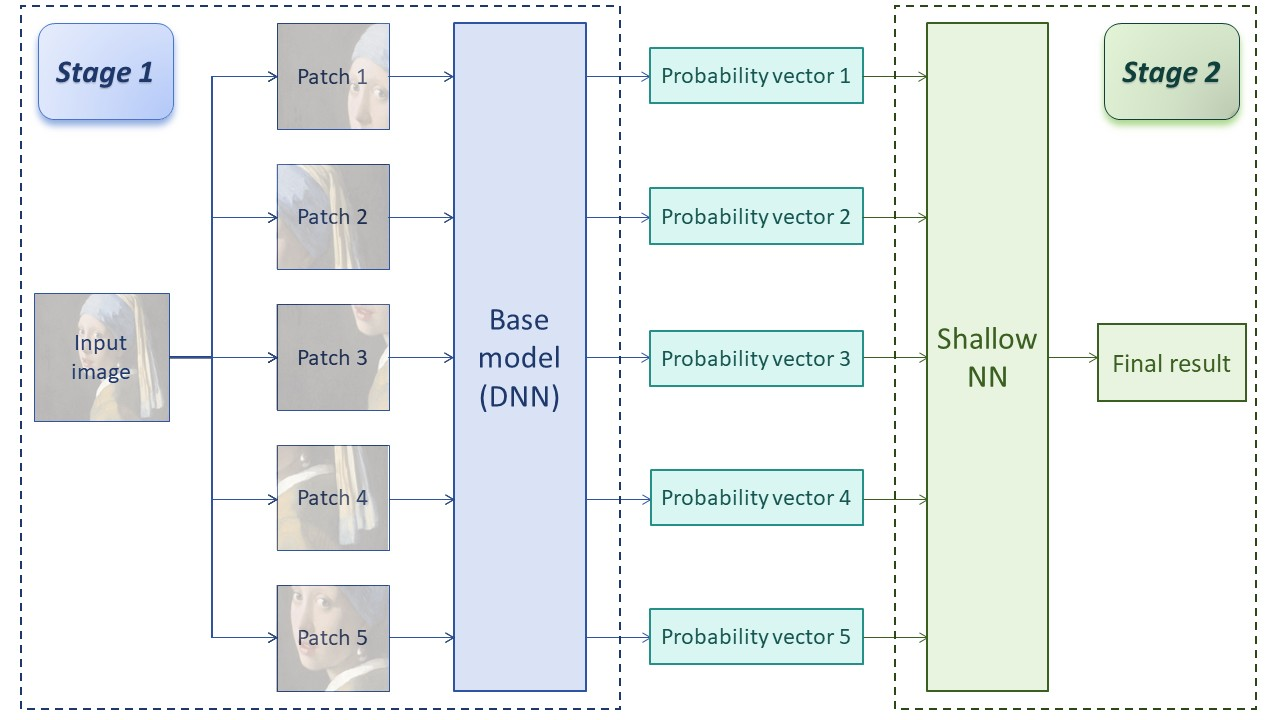
\includegraphics[width=0.5\textwidth]{fig/mainpipline.jpg}
    \caption{The architecture of the basic SNN adapter}
    \label{fig:architecture}
\end{figure}
The prediction consist of 2 stages. At the first stage, the image is dividing into 5 patches, as shown in Figure \ref{fig:patches}. The DNN independently 
classifies each of these five patches. In the second stage, the SNN functions as a decision-maker:  it takes the 
probability distributions generated by the DNN for the five patches as input and produces the final classification result.
\begin{figure}[h]
    \centering
    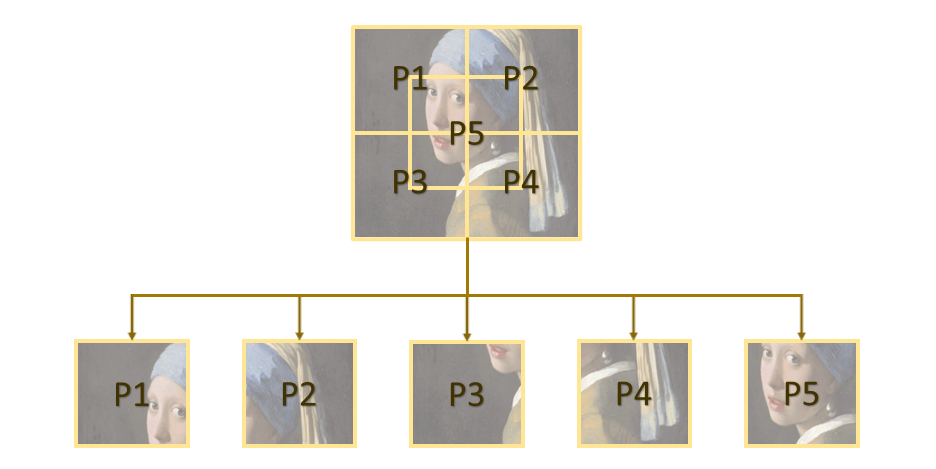
\includegraphics[width=0.5\textwidth]{fig/patch.png}
    \caption{Patch dividing of each image}
    \label{fig:patches}
\end{figure}

The proposed two-stage architecture combining a DNN and an SNN offers several key advantages:
\begin{itemize}
    \item It enables a more detailed examination of different regions within an artwork. By capturing fine-grained information and preserving important artistic details, this architecture enhances classification accuracy\cite{imran2023artistic}.
    \item Using probability vectors instead of images as inputs to the SNN reduces computational costs and avoids potential errors during image processing.
    \item The SNN functions as an independent decision-making adapter, making the model more flexible and generalizable. Since the DNN and SNN are trained independently, we can adjust their weights and architectures according to our needs. Each SNN adapter can fit different kinds of DNN models.
\end{itemize}

\subsection{Hierarchy SNN Architecture}
Despite the strong performance of the basic SNN adapter, it still faces certain limitations. Upon comparing the comprehensive prediction results of the DNN direct output and the SNN adapter output, we observed that while the SNN achieves higher overall accuracy, the DNN direct prediction exhibits superior accuracy in certain specific classes. 

To integrate the strengths of both networks, we proposed a two-layer hierarchical classification architecture. This architecture aims to extract both global and local features to generate the final prediction. The prediction pipeline is illustrated in Figure \ref{fig:hierarchical}.
\begin{figure}[h]
    \centering
    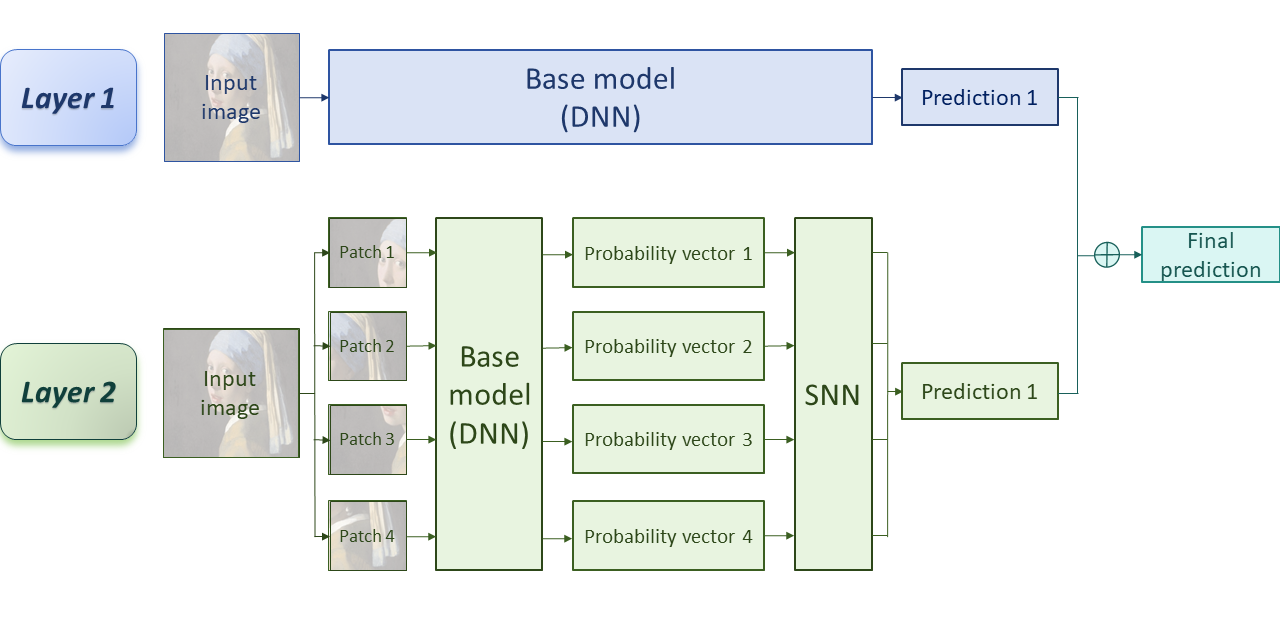
\includegraphics[width=0.5\textwidth]{fig/hierarchy.png}
    \caption{The architecture of the hierarchical SNN adapter}
    \label{fig:hierarchical}
\end{figure}

In this architecture, we employ a two-layer prediction scheme. In the first layer, the input image is fed directly into the base model (DNN), yielding the layer 1 prediction $p_{\text{layer1}}$ 
in the form of a probability vector. In the second layer, the input image is divided into four patches: left-top, left-bottom, right-top, and right-bottom. The DNN independently classifies each of these patches, generating probability vectors $p_1,p_2,p_3,p_4$. These probability vectors are then fed into the SNN adapter, which produces the layer 2 prediction 
$p_{\text{layer2}}$, also in the form of a probability vector.

The final prediction is a weighted sum of the predictions from the two layers:
\begin{align}
    p_{\text{final}} = w_1\cdot p_{\text{layer1}} + w_2\cdot p_{\text{layer2}},
\end{align}
where the weights $w_1$ and $w_2$ are proportional to the "reliability" of the respective layers. 
As suggested in \cite{hua2020artist}, the "reliability" can be evaluated based on the entropy of the probability vectors. Specificly, 
the entropy of the layer 1 prediction is calculated as:
\begin{align}
    H^1 &= -\sum_{i=1}^{C} p_{\text{layer1}}(i) \cdot \log(p_{\text{layer1}}(i)),
\end{align}
and the corresponding weight $w_1$ is given by:
\begin{align}
    w_1 &= 1 + 1/\exp(H^1),
\end{align}
For the second layer, the average probability vector $\overline{p}_{\text{layer2}}$ is fist computed as:
\begin{align}
    \overline{p}_{\text{layer2}}&=\frac{1}{4}(p_1 + p_2 + p_3 + p_4).
\end{align}
The entropy of the average probability vector is then calculated as:
\begin{align}
    H^2 &= -\sum_{i=1}^{C} \overline{p}_{\text{layer2}}(i) \cdot \log(\overline{p}_{\text{layer2}}(i)),
\end{align}
and the corresponding weight $w_2$ is given by:
\begin{align}
    w_2 &= 1 + 1/\exp(H^2).
\end{align}

\subsection{Patch Selection for SNN}

\section{Experiment}
\label{sec:experiment}
In this section, we present an comprehensive evaluation of our proposed method.
\subsection{Experiment Setup}
\subsubsection{Dataset}We utilize the Painter by Numbers dataset \cite{painter_by_numbers} as
the primary source of paintings for our study. This dataset is a vast collection of approximately 23,000 unique paintings, each labeled with the painter's name, style (or movement), genre, and additional information\cite{artnet}. For each experiment, we select a subset of 4,000 to 5,000 paintings from the training data. Additionally, we use 500 paintings from the test set for evaluation purposes.
\subsubsection{Evaluation}In order to get a comprehensive understanding of the model's performance, we evaluate the model using four metrics: accuracy, precision, recall and F1 score. 
\begin{itemize}
    \item \textbf{Accuracy:} The ratio of correctly predicted instances to the total instances in the dataset.
    \item \textbf{Precision:} The ratio of true positive predictions to the total predicted positives. It indicates the quality of the positive predictions.
    \item \textbf{Recall:} The ratio of true positive predictions to the total actual positives. It measures the model's ability to identify all relevant instances.
    \item \textbf{F1 Score:} The harmonic mean of precision and recall. It provides a balance between precision and recall, especially useful when dealing with imbalanced datasets.
\end{itemize}
Moreover, we not only evaluate the overall model performance but also analyze each class's performance. This provides deeper insights into the model's strengths and weaknesses across categories, helping identify specific areas needing improvement and ensuring consistent performance across all classes.
\subsubsection{Baseline DNN Architecture}We evaluate out SNN adapter on 3 various already-trained DNN models, \textit{DenseNet-121, VGG-19, and ResNet-50}. 
\begin{itemize}
    \item \textbf{DenseNet-121:} We adopt ArtNet model\cite{artnet} trained with DenseNet-121 architecture as our first baseline A key feature of ArtNet is its preprocessing
strategy, where each input image is first padded to a uniform
size and then divided into five patches. Both the full image
and its patches are included in the training set, enabling the
model to learn from global composition as well as local texture details, making it 
a perfect choice for our baseline model.
\item \textbf{VGG-19:} We utilize the model trained by \cite{qchaldemer2023paintingclassification} as our baseline for VGG-19. This model is trained on the same dataset as our method, with a test accuracy lower than ArtNet.
\item \textbf{ResNet-50:} We also employ the pretrained ResNet-50 model from \cite{kayracoskun2023artstyleclassification}. Our results show that even if the base model's performance is subpar, the SNN adapter can still significantly enhance the overall performance.
\end{itemize}

\subsection{Basic SNN Architecture}
We compare the DNN + patch-based SNN adapter architecture with two other approaches: the baseline DNN model and the patch-based DNN model. The patch-based DNN model generates predictions by averaging the five patch predictions.

\subsection{Hierarchy SNN Architecture}


\section{Patch Dividing}

{
    \small
    \bibliographystyle{ieeenat_fullname}
    \bibliography{main}
}

% WARNING: do not forget to delete the supplementary pages from your submission 
% \input{sec/X_suppl}

\end{document}
